\section{Реализация}
\subsection{Онтологии для замены неизвестных слов}\label{ontology}
Способ содержательного устранения проблемы с неизвестностью слов в анализируемых примерах,
предлагаемый в работе, --- это использование онтологий. Онтологией называется некоторая схема области
знаний, обычно она представляет собой направленный ациклический граф, вершины которого ---
понятия. Чем выше в графе находится вершина, тем шире соответствующее ей понятие. Таким образом,
если в сообщении встретилось слово, которое классификатору неизвестно, его можно заменить на более
общее понятие в соответствии с онтологией.

База знаний Википедии\footnote{https://www.wikipedia.org/} составляется пользователями и на данный
момент содержит 4515000 статей только на английском языке. Структура организации статей в
Википедии похожа на то, что мы ищем, --- это граф категорий.
На основе категорий Википедии уже составлена онтология проектом DBpedia\cite{dbpedia-swj} --- она и
используется в работе.

Данные выкачиваются в формате
Turtle\footnote{http://www.w3.org/TR/turtle/}. У нас есть два файла: первый --- отображение статей в
подмножество категорий, второй --- лес всех категорий. Граф категорий сильно несвязный, большинство
из них не участвуют ни в какой иерархии. Согласно этим особенностям нужно решить задачу хранения
онтологии и поиска нужной категории.

В первую очередь, стоит сказать, что хранится отображение категорий в номера вершин в графе, так как
хранить целые строчки для такого количества данных неэкономно. Эти отображения кладутся в
бор\footnote{Marisa trie: https://code.google.com/p/marisa-trie/}, в
соседнем боре запоминаются отображения статей в категории. Пример можно увидеть на рисунке \ref{ontology}.
Когда появляется неизвестное слово, ищется статья, где искомое
слово --- префикс, так как названия статей не всегда из одного слова.
Выбираем из всех категорий, к которым относится данная статья, ту, что в иерархии находится ниже всего. При равенстве уровня выбираем любую.

\begin{figure}
  \centering
  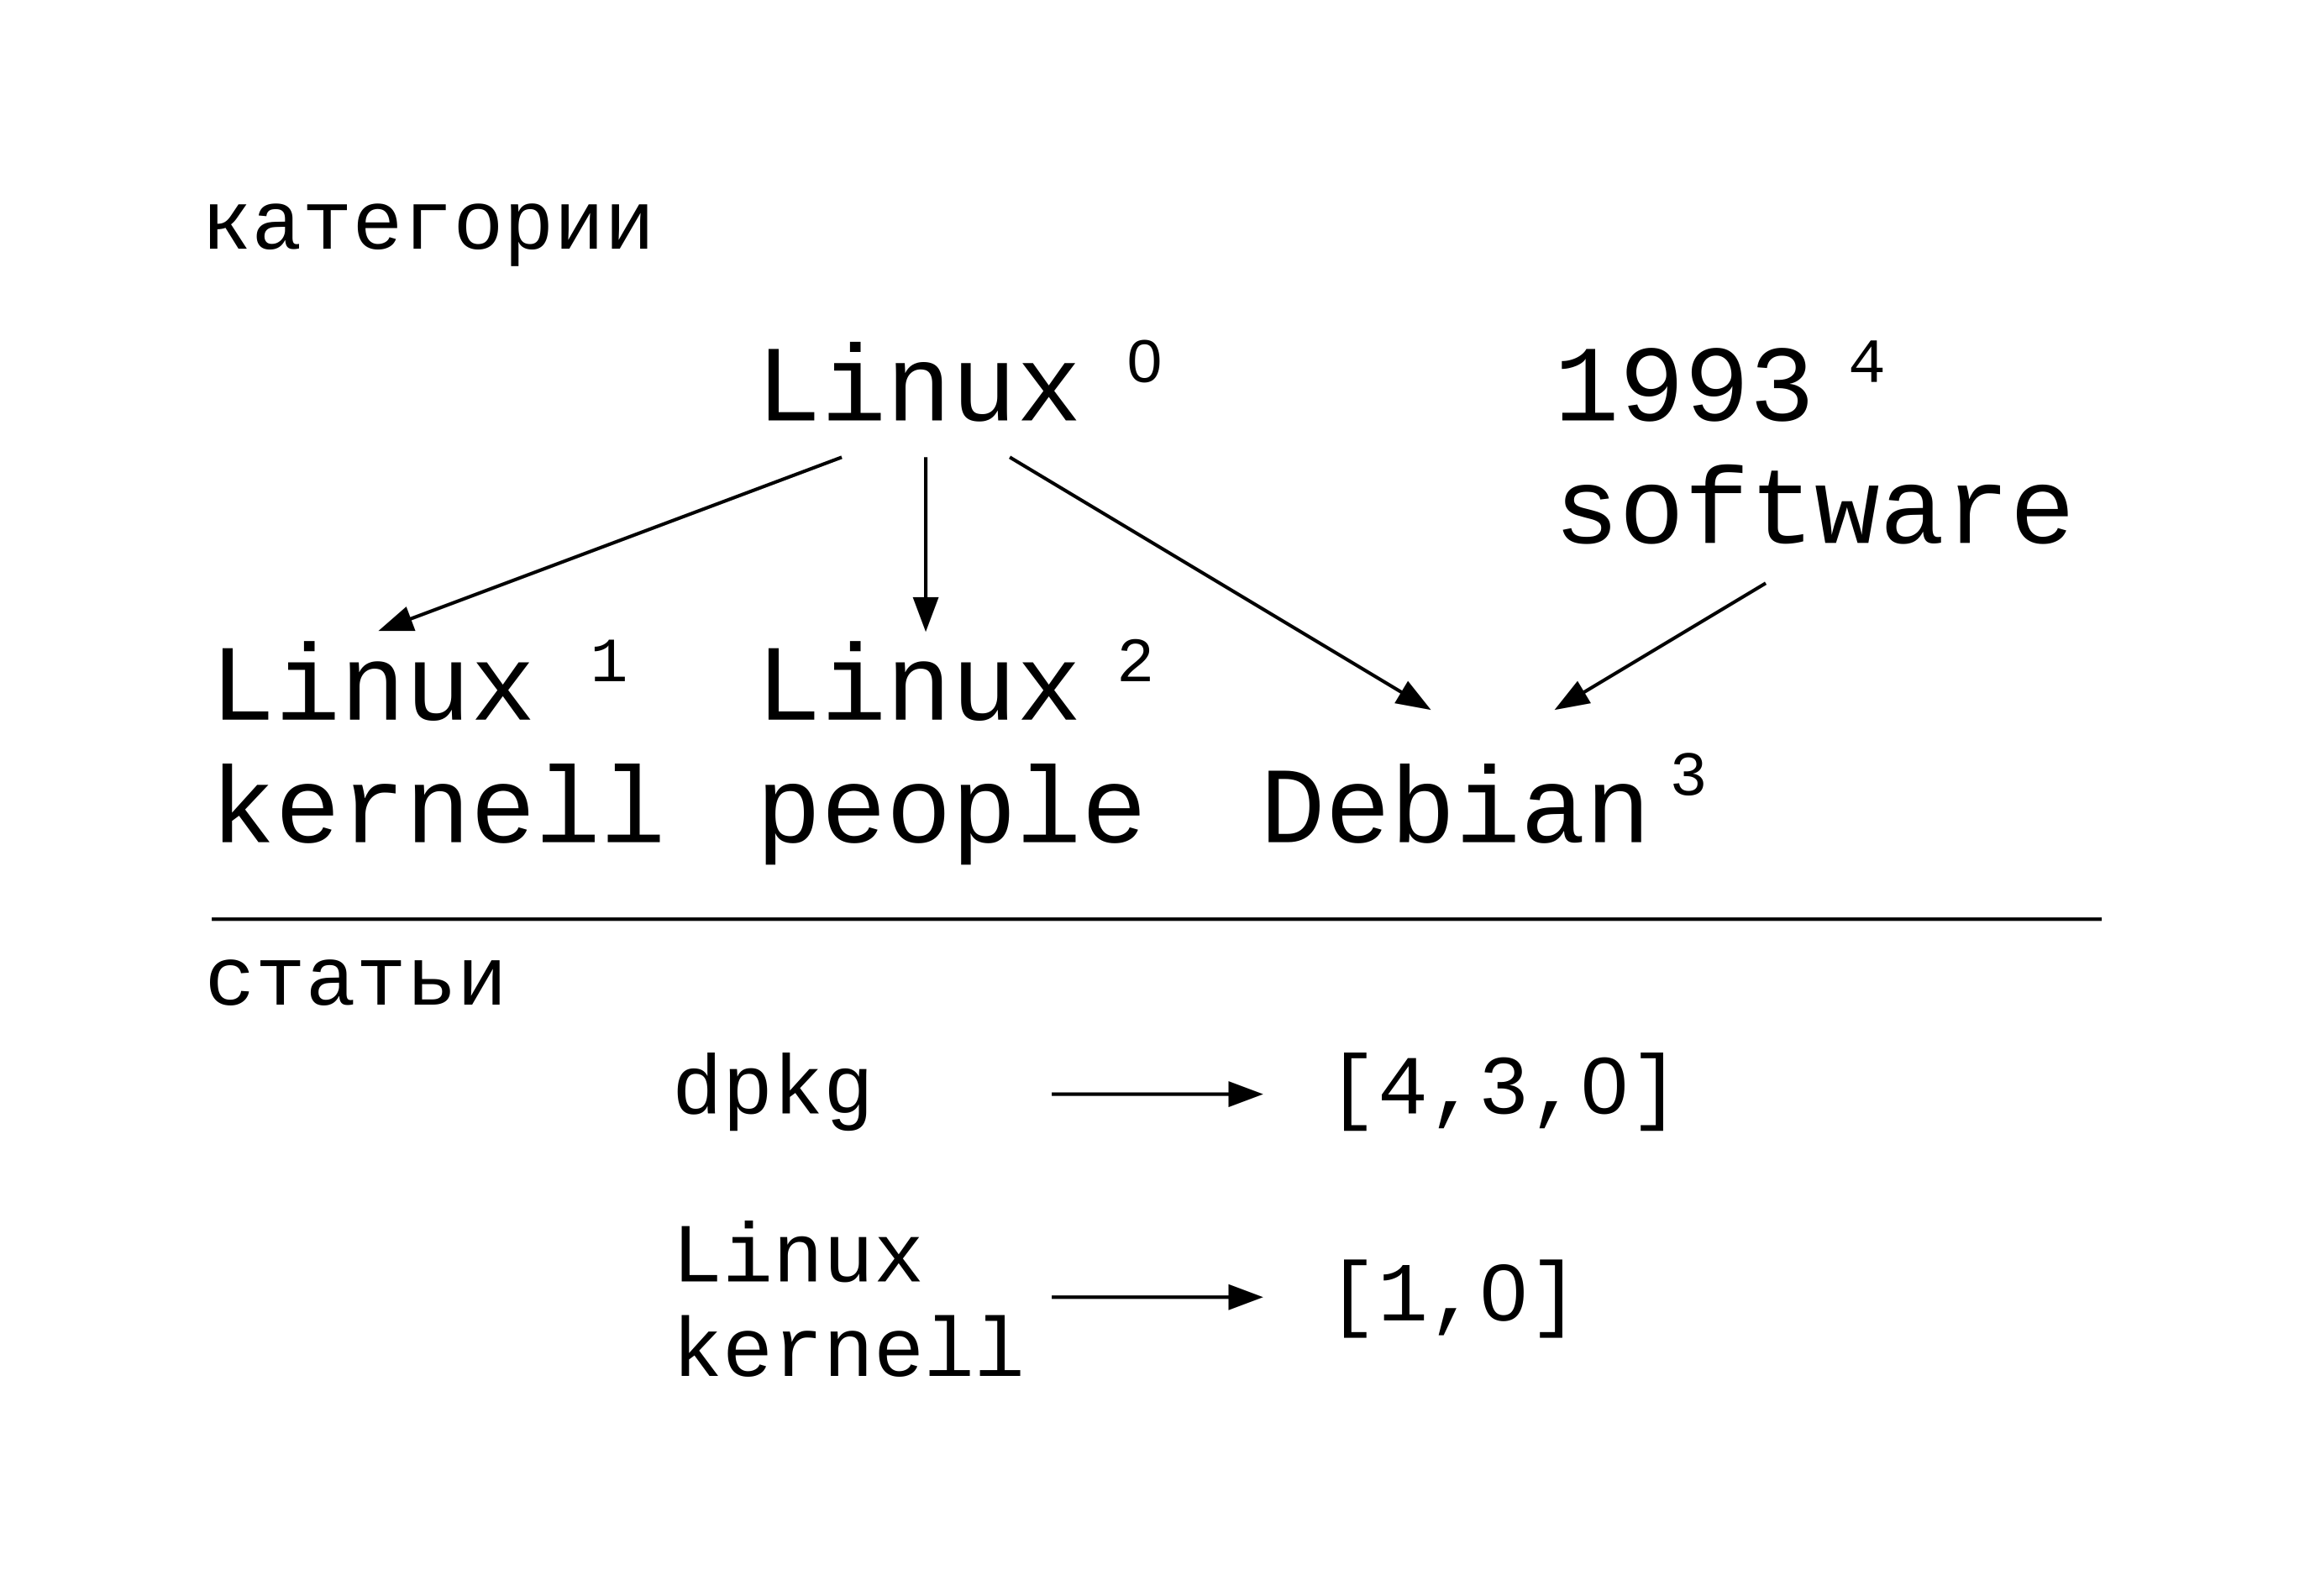
\includegraphics[width=0.5\textwidth]{ontology}
  \caption{Хранение статей <<Linux kernell>> и <<dpkg>> с некоторыми связанными с ними категориями.
Сверху -- бор категорий, снизу -- отображения статей. <<Linux kernell>> здесь
присутствует два раза, так как есть такая категория и одноимённая ей статья.}\label{ontology}
\end{figure}

\subsection{Алгоритмы подготовки данных, предсказывания и обучения}
Описанные в ходе данной работы идеи были объединены в метод классификации
и реализованы на языке Python с использованием его расширения Cython. Ниже
приведена последовательность действий со ссылками на разделы в тексте, где про эти действия
рассказывается более подробно. Некоторые моменты не были разъяснены ранее, поэтому им уделяется чуть
больше внимания. Отдельно рассмотрим три части: подготовка данных, обучение классификатора,
предсказание класса.

\textbf{Подготовка данных} (некоторые пункты не относятся к данным из обучающей выборки, в этом
случае в конце пункта стоит <<*>>):
\begin{itemize}
  \setlength{\itemsep}{1pt}%
    \setlength{\parskip}{1pt}
  \item замена сущностей html на слово <<URL>>, упоминаний пользователя на <<USER>> и чисел на <<42>>;
  \item перевод сообщения в нижний регистр;
  \item замена смайлов, хештегов и некоторых знаков препинания на <<+>> или <<$\minus$>> (раздел \ref{spec});
  \item замена долгого повторения гласных на сочетание из двух букв (раздел \ref{spec});
  \item разбивка на слова с учётом знаков препинания при помощи Penn Treebank Tokenizer из NLTK\cite{bird2006nltk};
  \item замена сокращений на их расшифровки (раздел \ref{spec});
  \item замена неизвестных классификатору слов на обобщения каждого из них (раздел \ref{ontology});*
  \item приведение всех слов к начальной форме при помощи алгоритма Snowball
  Stemmer\cite{porter2001snowball}
  \item удаление артиклей, предлогов и союзов из сообщения.
\end{itemize}

\textbf{Обучение классификатора:}
\begin{itemize}
  \setlength{\itemsep}{1pt}%
    \setlength{\parskip}{1pt}
\item подготовка данных и сохранение множества известных слов;
\item преобразование полученных строк на перекрывающиеся пары триграмм\footnote{Из предложения
    \texttt{\textbf{Мама\_мыла\_раму.}} получатся следующие пары триграмм: \texttt{\textbf{Мам|а\_м}},
    \texttt{\textbf{а\_м|ыла}}, \texttt{\textbf{ыла|\_ра}}, \texttt{\textbf{\_ра|му.}}}, теперь одна пара триграмм --- это признак, по которому измеряются сообщения;
\item каждый пример из обучающей выборки преобразуется в числовой вектор: на месте соответствующей
  пары триграмм из набора ставится $1$, если она есть в примере, и $0$, если нет;
\item поиск апостериорных распределений параметров согласно формулам \ref{eq:pi} и \ref{eq:thetajkc}.
\end{itemize}

\begin{samepage}
  \textbf{Предсказание класса для нового примера:}
  \begin{itemize}
    \setlength{\itemsep}{1pt}%
    \setlength{\parskip}{1pt}
  \item подготовка примера согласно описанному выше в <<Подготовка данных>>;
  \item преобразование полученной строки на перекрывающиеся пары триграмм;
  \item преобразование полученного набора в числовой вектор: на месте соответствующей
    пары триграмм из набора ставится $1$, если она есть в примере, и $0$, если нет;
  \item вычисление вероятности примера оказаться в каждом из классов (<<$1$>> или <<$-1$>>) согласно выражению
    \ref{eq:bnbpred} и вычислению множителей из неё по \ref{eq:mathpi3} и \ref{eq:maththetagr}
  \item выбор класса, который дал наибольшую вероятность попадания в него.
  \end{itemize}
\end{samepage}
